\documentclass[tikz,border=2mm]{standalone}
\tikzset{global scale/.style={
    	scale=#1,
    	every node/.append style={scale=#1}
  	}
}
\begin{document}
	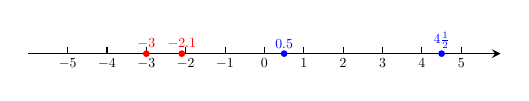
\begin{tikzpicture}[global scale = 0.5]
  		\draw [black, ->, >=stealth] (-6,0) -- (6,0); % ->��ͷ��,>=stealth��ʵ�ļ�ͷ
		%\foreach \x in {-9, -8, -7, -6, -5, -4, -3, -2, -1, 0, 1, 2, 3, 4, 5, 6, 7, 8, 9}
		\foreach \x in {-5, ..., 5}
			\draw (\x cm,5pt) -- (\x cm,0pt) node[anchor=north] {$\x$};
		% (1) - 2.1, - 3, 0.5, 4+1/2; ������������(2) - 50, 250, 0, - 400
		\draw [red, fill=red] (-2.1, 0) circle(2pt) node [above] {$-2.1$}; 
		\draw [red, fill=red] (-3, 0) circle(2pt) node [above] {$-3$}; 	
		\draw [blue, fill=blue] (0.5, 0) circle(2pt) node [above] {$0.5$}; 
		\draw [blue, fill=blue] (4+1/2, 0) circle(2pt) node [above] {$4\frac{1}{2}$}; 		
		
		
	\end{tikzpicture}    
\end{document}
